\documentclass[tikz,border=2pt]{standalone}
\usepackage{amsmath}
\usepackage{sfmath}
\usetikzlibrary{arrows.meta,calc}

\begin{document}

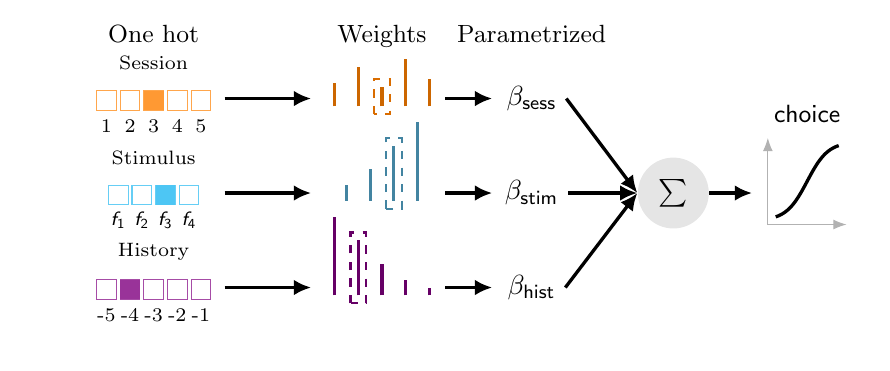
\begin{tikzpicture}[
    font=\sffamily,
    >=Latex,
    arrow/.style={very thick,-{Latex[length=2.2mm,width=2mm]}},
    sum/.style={
      circle,
      minimum size=0.9cm,
      fill=gray!20,
      draw=none,
      font=\bfseries
    }
  ]

  \path[use as bounding box] (0,-2.0) rectangle (10.6,2.0);

  % Row anchors
  \def\ySess{1.2}
  \def\yStim{0.0}
  \def\yHist{-1.2}

  % =====================================================
  % COLUMN CENTERS (THIS FIXES EVERYTHING)
  % =====================================================
  \def\xOneHotC{1.6}
  \def\xWeightsC{4.5}
  \def\xParamC{6.4}

  \def\smallGap{1.2}
  \def\xSigma{\xParamC + 1.5*\smallGap}
  \def\xPsych{\xSigma + \smallGap}

  % Geometry
  \def\boxW{0.25}
  \def\boxStep{0.3}

  % Starts so each row is centered
  \def\xSessStart{\xOneHotC - 0.725} % 5 boxes
  \def\xStimStart{\xOneHotC - 0.575} % 4 boxes
  \def\xHistStart{\xOneHotC - 0.725}

  % Weight starts
  \def\xSessWStart{\xWeightsC - 0.6}
  \def\xStimWStart{\xWeightsC - 0.45}
  \def\xHistWStart{\xWeightsC - 0.6}

  % =====================================================
  % COLUMN TITLES
  % =====================================================
  \node[font=\small, text height=1.5ex, text depth=0.25ex]
  at (\xOneHotC,1.9) {One hot};

  \node[font=\small, text height=1.5ex, text depth=0.25ex]
  at (\xWeightsC,1.9) {Weights};

  \node[font=\small, text height=1.5ex, text depth=0.25ex]
  at (\xParamC,1.9) {Parametrized};

  % =====================================================
  % ROW LABELS
  % =====================================================
  \node[font=\scriptsize] at (\xOneHotC,\ySess+0.35) {Session};
  \node[font=\scriptsize] at (\xOneHotC,\yStim+0.35) {Stimulus};
  \node[font=\scriptsize] at (\xOneHotC,\yHist+0.35) {History};

  % =====================================================
  % ONE-HOT
  % =====================================================

  % Session
  \foreach \i/\lab in {0/1,1/2,2/3,3/4,4/5}{
    \pgfmathsetmacro{\x}{\xSessStart + \boxStep*\i}
    \draw[orange!70] (\x,\ySess) rectangle (\x+\boxW,\ySess-0.25);
    \node[font=\scriptsize] at (\x+0.5*\boxW,\ySess-0.45) {\lab};
  }
  \fill[orange!80] (\xSessStart+0.6,\ySess) rectangle
  (\xSessStart+0.6+\boxW,\ySess-0.25);

  % Stimulus
  \foreach \i/\lab in {0/$f_1$,1/$f_2$,2/$f_3$,3/$f_4$}{
    \pgfmathsetmacro{\x}{\xStimStart + \boxStep*\i}
    \draw[cyan!60] (\x,\yStim) rectangle (\x+\boxW,\yStim-0.25);
    \node[font=\scriptsize] at (\x+0.5*\boxW,\yStim-0.45) {\lab};
  }
  \fill[cyan!70] (\xStimStart+0.6,\yStim) rectangle
  (\xStimStart+0.6+\boxW,\yStim-0.25);

  % History
  \foreach \i/\lab in {0/-5,1/-4,2/-3,3/-2,4/-1}{
    \pgfmathsetmacro{\x}{\xHistStart + \boxStep*\i}
    \draw[violet!70] (\x,\yHist) rectangle (\x+\boxW,\yHist-0.25);
    \node[font=\scriptsize] at (\x+0.5*\boxW,\yHist-0.45) {\lab};
  }
  \fill[violet!80] (\xHistStart+0.3,\yHist) rectangle
  (\xHistStart+0.3+\boxW,\yHist-0.25);

  % =====================================================
  % WEIGHTS
  % =====================================================

  \foreach \i/\h in {0/0.3,1/0.5,2/0.25,3/0.6,4/0.35}{
    \pgfmathsetmacro{\x}{\xSessWStart + \boxStep*\i}
    \draw[orange!80!black, line width=1.2pt] (\x,\ySess-0.2) --
    (\x,\ySess-0.2+\h);
  }

  \foreach \i/\h in {0/0.2,1/0.4,2/0.7,3/1.0}{
    \pgfmathsetmacro{\x}{\xStimWStart + \boxStep*\i}
    \draw[cyan!60!black, line width=1.2pt] (\x,\yStim-0.2) --
    (\x,\yStim-0.2+\h);
  }

  \foreach \i/\h in {0/1.0,1/0.7,2/0.4,3/0.2,4/0.1}{
    \pgfmathsetmacro{\x}{\xHistWStart + \boxStep*\i}
    \draw[violet!80!black, line width=1.2pt] (\x,\yHist-0.2) --
    (\x,\yHist-0.2+\h);
  }

  % =====================================================
  % SELECTION
  % =====================================================
  \draw[dashed, thick, orange!85!black]
  (\xSessWStart+0.6-0.1,\ySess-0.3) rectangle
  (\xSessWStart+0.6+0.1,\ySess+0.15);

  \draw[dashed, thick, cyan!60!black]
  (\xStimWStart+0.6-0.1,\yStim-0.3) rectangle (\xStimWStart+0.6+0.1,\yStim+0.6);

  \draw[dashed, thick, violet!80!black]
  (\xHistWStart+0.3-0.1,\yHist-0.3) rectangle (\xHistWStart+0.3+0.1,\yHist+0.6);

  % =====================================================
  % ARROWS
  % =====================================================

  \draw[arrow] (\xOneHotC+0.9,\ySess-0.1) -- (\xWeightsC-0.9,\ySess-0.1);
  \draw[arrow] (\xOneHotC+0.9,\yStim-0.1) -- (\xWeightsC-0.9,\yStim-0.1);
  \draw[arrow] (\xOneHotC+0.9,\yHist-0.1) -- (\xWeightsC-0.9,\yHist-0.1);

  \draw[arrow] (\xWeightsC+0.8,\ySess-0.1) -- (\xParamC-0.5,\ySess-0.1);
  \draw[arrow] (\xWeightsC+0.8,\yStim-0.1) -- (\xParamC-0.5,\yStim-0.1);
  \draw[arrow] (\xWeightsC+0.8,\yHist-0.1) -- (\xParamC-0.5,\yHist-0.1);

  % =====================================================
  % GLM + SIGMA
  % =====================================================

  \node (b1) at (\xParamC,\ySess-0.1) {$\beta_{\rm sess}$};
  \node (b2) at (\xParamC,\yStim-0.1) {$\beta_{\rm stim}$};
  \node (b3) at (\xParamC,\yHist-0.1) {$\beta_{\rm hist}$};

  \node[sum] (sum) at (\xSigma,\yStim-0.1) {$\sum$};

  \draw[arrow] (b1.east) -- (sum.west);
  \draw[arrow] (b2.east) -- (sum.west);
  \draw[arrow] (b3.east) -- (sum.west);

  \draw[arrow] (sum.east) -- (\xPsych-0.2,\yStim-0.1);

  % =====================================================
  % SIGMOID
  % =====================================================

  \draw[gray!60,->] (\xPsych,\yStim-0.5) -- (\xPsych+1.0,\yStim-0.5);
  \draw[gray!60,->] (\xPsych,\yStim-0.5) -- (\xPsych,\yStim+0.6);

  \def\sigmoid(#1){1/(1+exp(-#1))}
  \draw[very thick, domain=-3:3, samples=80]
  plot ({\xPsych+0.1 + 0.8*(\x+3)/6}, {\yStim-0.45 + 1.0*\sigmoid(\x)});

  \node at (\xPsych+0.5,\yStim+0.9) {\small choice};

\end{tikzpicture}
\end{document}